\documentclass[titlepage]{article}
\usepackage[norsk]{babel}
\usepackage[utf8]{inputenc}
%\usepackage[latin1]{inputenc}
\usepackage{graphicx}
\usepackage{float}
\usepackage{parskip}
\usepackage{array}
\newcolumntype{L}[1]{>{\raggedright\let\newline\\\arraybackslash\hspace{0pt}}m{#1}}
\newcolumntype{C}[1]{>{\centering\let\newline\\\arraybackslash\hspace{0pt}}m{#1}}
\newcolumntype{R}[1]{>{\raggedleft\let\newline\\\arraybackslash\hspace{0pt}}m{#1}}
\usepackage{longtable}

\author{Gruppe 38}
\title{KTN 1}
\date{\today}

\begin{document}

\maketitle

\tableofcontents

\newpage
\section{Innledning}
Vi skal tilby en forbindelsesorientert nettverksløsning, og dette skal vi gjøre ved hjelp av A1 og A2. A2 eksisterer allerede og er et forbindelsesløst nett. All kontakt mellom klienten og serveren for kalenderapplikasjonen vår skal gå igjennom A1, som deretter tar kontakt med A2 (socketen). Tilkoblingen mot A1 skal være pålitelig og tapsfri, akkurat som TCP. Vi skal endre på ConnectionImpl-klassen som implementerer Connection-klassen. Det er 4 sentrale metoder vi skal impelentere. Disse er accept(), connect(address, port), close(), send() og receive(). Om vi skulle ønske, og ha behov, kan vi også implementere isValid(packet). A1 skal kommunisere med A2 gjennom metodene send, receive og cancel\_receive som ligger i A2.

For å kunne opprette en pålitelig tilkopling igjennom A2, må vi selv opprette koplinger for data som skal sendes. Når dette er gjort kan vi sikre tapsfri overføring. I sekvensdiagrammene vi har laget, viser vi hvordan serveren og klienten kan abstrahere bort mange funksjoner som alltid må kjøres, og dermed bare konsentrere seg om det essensielle. Vi viser spesifikt tilfellene Connect, Send og Close.

Når vi oppretter en connection skal det utføres en three-way-handshake. Først sender vi en SYN fra klienten til servern, i respons får vi en SYN-ACK tilbake, og tilslutt sender klienten en ACK til servern og det har blitt dannet en tilkobling.

Hver gang en pakke blir sendt så sender man med et sekvensnummer, deretter får man tilbake en ACK og hva mottakeren forventer at neste sekvensnummer skal være, dermed vet man at pakken kom fram. 
Når en tilkobling skal bli lukket vil det utføres en three-way-handshake her også. Dette foregår ved at klienten sender en FIN mot servern, som vil svare med ACK (servern har fått pakken) og en FIN selv. Klienten får dette tilbake og svarer da med en ACK selv, og tilkoblingen blir avsluttet.
For å kunne lage en god kommunikasjon, er det fint å vite hva som finnes i A2. Dette kan aksesseres ved å bruke Admin-klassen. Vi kan her skrive ut logger fra A2 og gjøre innstillinger. Med disse verktøyene kan vi lage en pålitelig og god tilkopling.

\newpage
\section{Feilhåndtering}
\textbf{Beskrivelsen av A2 tilsier at det kan oppstå fire forskjellige typer feil med tanke på pakkeoverføring. Vi skal implementere A1, som skal behandle, og rette opp disse feilene.}

\subsection{Package lost}
Hvis senderen ikke mottar en ACK før den når timeout-tiden vil en pakke bli regnet som tapt.
Pakker med lavere sekvensnummer blir regnet som tapt hvis sekvensnummeret vi mottar er høyere enn forventet. 
Hvis dette skjer vil samme pakke bli sendt på nytt, helt til senderen mottar en ACK før timeout-tiden, og får forventet sekvensnummer tilbake.
Metoden sendDataPacketWithRetransmit() i klassen AbstractConnection gjør akkurat dette for oss. 

\subsection{Package delayed}
Hvis mottakeren sender ACK to ganger for samme pakke, betyr det at pakken har blitt sendt to ganger fordi den første ikke kom fram raskt nok.
Dette har ikke noe å si for senderen, han vil bare ignorere den andre ACKen. Mottakeren vil ignorere en pakke han allerede har fått. 
 
\subsection{Package has errors}
Vi må her sjekke om pakken mottatt er samme pakke som ble sendt og inneholder det samme sekvensnummeret. Vi kan her implementere isValid()-funksjonen for å gjøre dette. Her brukers checksumen som blir sendt med pakken for å sjekke om pakken inneholder feil.
 
\subsection{Ghost package}
Her er det snakk om en pakke ingen venter, som bare oppstår. Vi kan sjekke sekvensnummer, og bruke isValid()-funksjonen for å eliminere dette. 

\newpage
\section{Diagrammer}
\subsection{Sekvensdiagrammer}
\subsubsection{Connect}
\begin{figure}[H]
\label{fig:conSEQ}
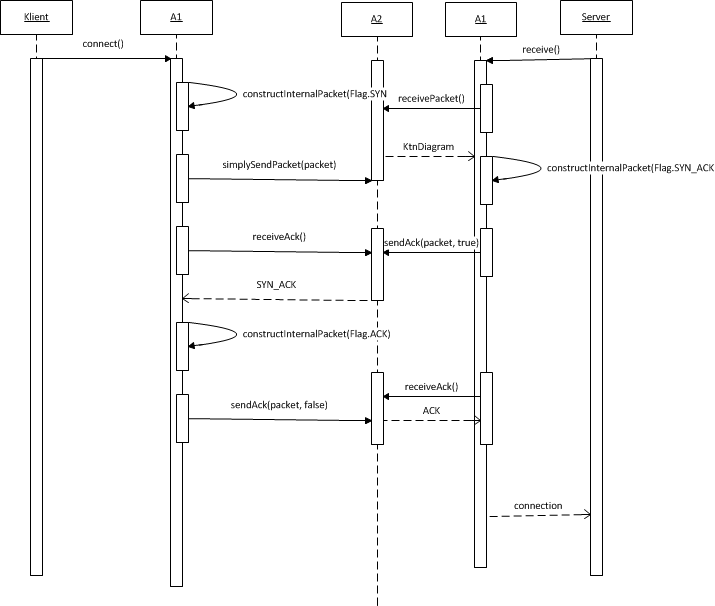
\includegraphics[width=400px]{connectSEQ.png}
\caption{Sekvensdiagram for connect()}
\end{figure}

\subsubsection{Send}
\begin{figure}[H]
\label{fig:sendSEQ}
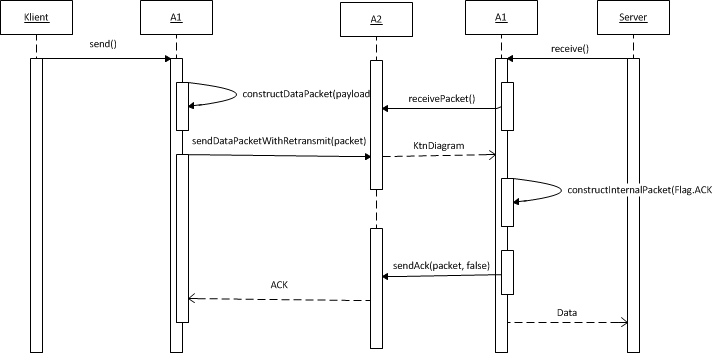
\includegraphics[width=400px]{sendSEQ.png}
\caption{Sekvensdiagram for send()}
\end{figure}

\subsubsection{Close}
\begin{figure}[H]
\label{fig:closeSEQ}
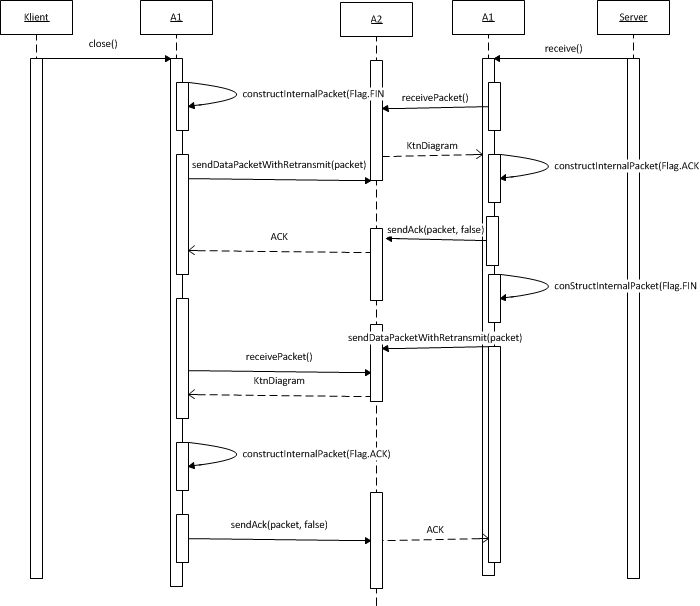
\includegraphics[width=400px]{closeSEQ.png}
\caption{Sekvensdiagram for close()}
\end{figure}

\subsection{Statediagrammer}
\subsubsection{Server}
\begin{figure}[H]
\label{fig:serverSTATE}
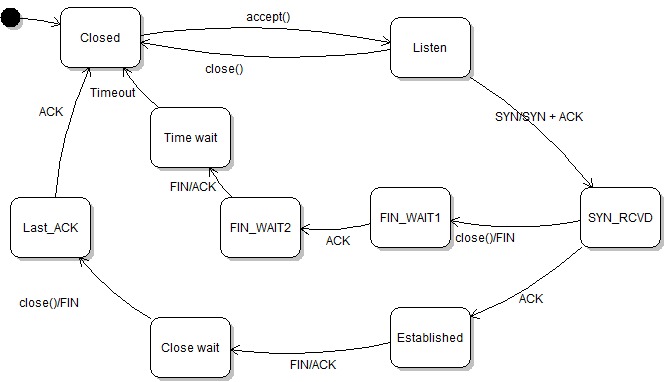
\includegraphics[width=400px]{serverSTATE.png}
\caption{Statediagram for server}
\end{figure}

\subsubsection{Klient}
\begin{figure}[H]
\label{fig:clientSTATE}
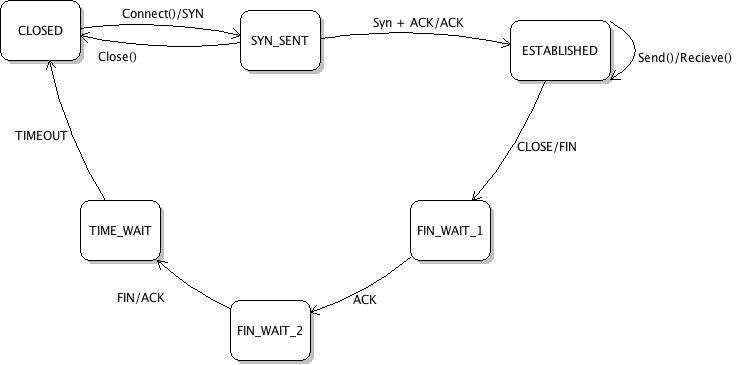
\includegraphics[width=400px]{clientSTATE.png}
\caption{Statediagram for klient}
\end{figure}

\newpage
\section{Testplan}
\subsection{Krav som skal testes}
Krav 1: Bruke Connection-klassen i applikasjonen
Krav 2: Kommunisere mellom A1 og A2 via send(), receive og cancel\_revceive()
Krav 3: A1 skal kunne kople fra, motta data og sende data til andre instanser.
Krav 4: Alle feil som oppstår i A2, skal tas hånd om i A1

\subsection{Krav 1 og 2}
Vi skal bruke Connection-klassen for å kommunisere med applikasjonen, og A1 kan kun kommunisere med A2 gjennom metodene beskrevet i Krav 2. 
Ettersom disse kravene må være oppfylt for at de andre funskjonene skal fungere vil vi ikke legge så mye vekt på å teste dem spesefikt, men disse kravene vil bli testet sammen med de andre kravene.

\subsection{Krav 3}
\subsubsection{Kople til}
Vi kan lage testcase for å sjekke at når du kopler til mellom klient og server. så blir en three-way-handshake gjennomført som beskrevet i sekvensdiagram \ref{fig:conSEQ}. Dette er blir da bare å sjekke at et SYN-flagg blir sendt, at det blir sendt tilbake SYN\_ACK-flagg og at det tilslutt blir sendt et ACK-flagg.

\subsubsection{Kople fra}
På samme måte som kople til, lager vi en testcase og bruker flaggene som skal bli sendt for å sjekke at det foregår på riktig måte. Senderen skal sende et FIN-flagg og få i retur et ACK-flagg og et FIN-flagg. Når senderen mottar dette sender han et ACK-flagg tilbake, og klienten blir koplet fra. Dette er beskrevet i sekvensdiagram \ref{fig:closeSEQ}.

\subsubsection{Motta / sende data}
Hvis man ser på sekvensdiagram \ref{fig:sendSEQ} ser man at hver gang data blir sendt skal mottaker svare med en ACK så senderen vet at pakken har kommet fram. Hvis senderen ikke mottar en ACK før timeout-tiden vil den sende pakken på nytt. Dette kan vi teste med en testcase hvor vi prøver å sende pakker, og se om vi mottar ACK og riktig forventet sekvensnummer fra mottaker.

\subsection{Krav 4}
Feil som kan forekomme i A2 har vi skrevet om i feilhåndtering \ref{fig:conSEQ}. Det er fire forskjellige feil det er snakk om og disse er, forsvunnet pakke, forsinket pakke, feil i pakke og ghostpakke. 
Alle de feilene skal vi håndtere i A1 og måten vi kan teste dette på er å bruke filen, Settings.xml i Admin-pakken, som gir oss mulighet til å sette sannsynligheter for hvor ofte hver feil skal forekomme. Samtidig som vi tester dette, må vi sjekke at hvis feil oppstår så er de usynlige for applikasjonen.

\subsubsection{Sannsynlighet for feil}
\begin{table}[H]
\centering
\label{tab:feilsan}
\begin{tabular}{| l | l | l | l | l |}
\hline
Testcase & Package lost & Package delayed & Package has errors & Ghost package \\
\hline
1 - Uten feil & 0 & 0 & 0 & 0 \\
\hline
2.1 & 0.1 & 0 & 0 & 0 \\
\hline
2.2 & 0.5 & 0 & 0 & 0 \\
\hline
3.1 & 0 & 0.1 & 0 & 0 \\
\hline
3.2 & 0 & 0.5 & 0 & 0 \\
\hline
4.1 & 0 & 0 & 0.1 & 0 \\
\hline
4.2 & 0 & 0 & 0.5 & 0 \\
\hline
5.1 & 0 & 0 & 0 & 0.1 \\
\hline
5.2 & 0 & 0 & 0 & 0.5 \\
\hline
6.1 - Kombinasjon & 0 & 0 & 0.5 & 0.5 \\
\hline
6.2 - Kombinasjon & 0.5 & 0.5 & 0.3 & 0 \\
\hline
7 - Alle feil & 0.5 & 0.5 & 0.5 & 0.5 \\
\hline
\end{tabular}
\caption{Tabell for feilsannsynlighet}
\end{table}

Vi vil kjøre testcasene i samme rekkefølge som tabellen fordi vi syns dette gir oss mest ut av testcasene. Før må vi sjekke at alt fungerer med ingen feil, så går vi systematisk igjennom hver av feilene som kan oppstå og først sjekker for 10 \% sannsynlighet og så 50 \% sannsynlighet.

\textbf{Testcase 6}:\\
I 6.1 har vi valgt å teste feil i pakken og ghostpakke med lik sannsynlighet for begge to, fordi da får vi sjekket om implementasjonen vår håndterer pakker som har feil i header-felt (ghostpakke) og feil i payloaden (feil i pakke). Grunnen til at vi har valgt 50 \% sannsynlighet for begge to, er fordi implementasjonen skal klare å håndtere begge feilene, og målet er at implementasjonen skal klare å håndtere feil opptil 50 \%. Det er bra å teste begge feilkategoriene sammen fordi de går ut på det samme, bare at feilen fins i forskjellige deler av pakken. 

I 6.2 tester vi at pakker er mistet og at pakker er forsinket i samme testcase fordi dette henger mye sammen. Senderen vil reagere på samme måte hvis en pakke er forsinket eller mistet, fordi da har timeout-tiden gått og den vil sende pakken på nytt. Det vi da tester er at mottakeren klarere å håndtere dupliserte pakker, altså at den bare tar vare på den ene pakken. Samtidig får vi testet at senderen faktisk sender ut en ny pakke, hvis den ikke mottar en ACK innenfor en gitt tidsramme. Grunnen til å ha med feil i pakke i samme testcase er fordi mottakeren må se etter feil også når pakken er forsinket. Vi valgte å ta en lavere sannsynlighet for feil i pakker, fordi vi først og fremst skal sjekke at vi håndterer forsinket og tapte pakker.

\textbf{Testcase 7}:\\
Vi har bestemt oss for at implementasjonen skal klare å håndtere minst 50 \% sannsynlighet for feil i hver kategori, og derfor har vi satt den sannsynligheten på hver feil som kan oppstå. Når denne testcasen er bestått vil vi prøve å øke sannsynligheten for feil i alle kategoriene for å kartlegge hvor stor prosentandel med feil implementasjonen vår tåler. 

\newpage
\listoftables

\newpage
\listoffigures

\newpage
\begin{thebibliography}{9}

\bibitem{fpkomp}
	Kompendium til fellesprosjektet,
	\emph{it's learning-gruppa til faget}
\end{thebibliography}

\end{document}
